\subsection{The PhaZor script}

To use PhaZor, all details of the task must be included in a \texttt{project.xml} script in order to specify the requested job. \\
\\
The first initial structure is a box-shaped structure with an input waveguide and two output waveguides (Fig.  \ref{fig:stanford}). The \texttt{design domain} is set as the inner box (Fig. \ref{fig:stanford_DD}). \\
\\
The \texttt{design domain} contains the region where the structure is to be optimised, i.e. the input and output waveguides are not changed during optimisation since they are outside the \texttt{design domain}. Since the FDTD method finds local solutions, the final design depends on the choice of initial structure. The \texttt{design domain} and initial structure are given to PhaZor as black and white .png files, with black representing inactive area (empty space) and white representing active area (filled space, in this case Si).\\
\\
The dimensions of the .png files match 1 pixel with 1 nm of the structure. The complete structure is within a defined \texttt{mesh} with a resolution of 40 nm. Each point on the \texttt{mesh} represents the volume encompassing the silicon structure, and these data points are subject to algorithm calculations. The resolution of 40 nm results in a manageable computation time with DTU's HPC cluster, while maintaining a precision high enough to obtain realistic results.\\
\\
The computation time needed to simulate 2D designs is much shorter compared to simulating 3D designs, so the structures were first simulated in 2D, i.e. the components in the \texttt{mesh} region were assumed to have no thickness. The promising structures and parameter values were then used in 3D simulations.\\
\\
The input waveguide is centered at ($-$2710 nm, 0 nm) with respect to the center of the structure, and the output upper and lower waveguides are centered at (2710 nm, 600 nm) and (2710 nm, $-$600 nm), respectively. When moving from 2D to 3D, the structure is given a thickness of 340 nm. The dimensions of structure can be seen on Fig. \ref{fig:initialBox} and Fig. \ref{fig:initialYjunction} (top-down views) and Fig. \ref{fig:initialside} (side-view).\\
\\
In reality the silicon structure is fabricated on a glass (SiO$_2$) surface. This glass surface has to be implemented in the script as well, as its material properties will influence the propagation of light through the demultiplexer component. The minimum feature size of the silicon structure is controlled with a filter size also specified in the script. Each material is defined through their permittivity $\epsilon_r$, permeability $\mu_r$, and conductivity $\sigma_r$, all relative to vacuum. For air; $(\epsilon_r, \, \mu_r, \, \sigma_r)=(1,1,0)$, and for Si; $(\epsilon_r, \, \mu_r, \, \sigma_r)=(11.38,1.0,0)$ in 3D. \\ 

Two Gaussian light pulses are emitted from the input waveguide with specified direction of propagation, temporal width, amplitude, and polarisation (in our case: TE-polarised). Since the optimisation depends on how these two light pulses propagate, the temporal width must be chosen so that the spectral width of the pulses overlap slightly. The optimised structure must able to handle the full spectrum of wavelengths, at least in the [1250, 1650] nm range.
\\\\

\begin{figure}[t]
    \centering
    \begin{subfigure}[h]{0.48\textwidth}
        \centering
        
\includegraphics[width=\textwidth]
        {fig/design/stanford.pdf}
        \caption{Initial box-shaped silicon structure.}
        \label{fig:stanford}
    \end{subfigure}
    \hspace{1mm}
    \begin{subfigure}[h]{0.48\textwidth}
        \centering
        
\includegraphics[width=\textwidth]
        {fig/design/stanford_Yjunction.pdf}
    \caption{Initial Y-junction-shaped silicon structure.}
    \label{stanford_Yjunction}
    \end{subfigure}
    \caption{The .png images loaded into PhaZor for the box structure and Y-junction structure. For dimensions of the structures (top-down view), see Fig. \ref{fig:initialBox} and Fig. \ref{fig:initialYjunction}. For a side-view, see Fig. \ref{fig:initialside}.}
    \label{fig:Inputfiles}
\end{figure}

\begin{figure}[h]
    \centering
    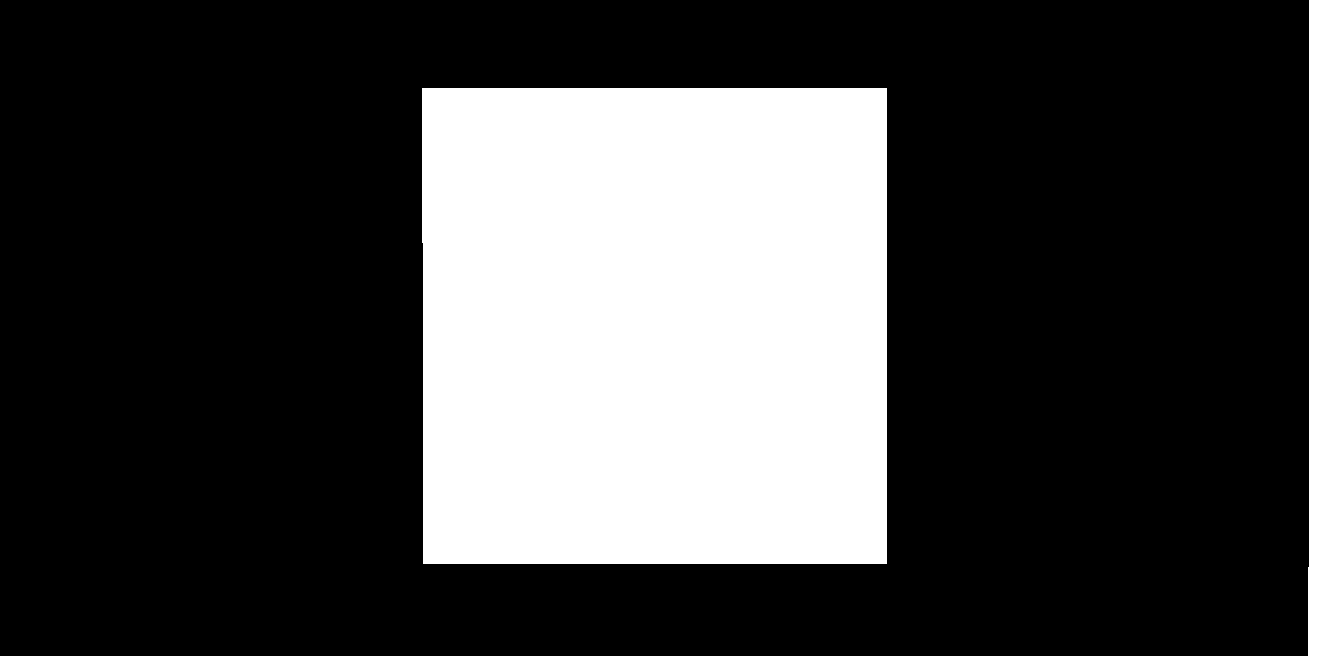
\includegraphics[width=0.48\textwidth]
        {fig/design/stanford_DD.pdf}
        \caption{\texttt{design domain} for all initial structures.}
        \label{fig:stanford_DD}
\end{figure}


\subsection{Chosen initial structures}
We chose to optimise six initial structures: Three box structures (Fig. \ref{fig:initialBox}), and three Y-junction structures (Fig. \ref{fig:initialYjunction}). The box-shaped design is meant to be the simplest initial design. Furthermore this design is what Stanford used as their initial design \cite{Stanford}, and in order to check our approach compared to theirs, this is the best suited initial design for that purpose. The solutions from the box-shaped structures all turned out to resemble Y-junctions, so by choosing a Y-junction shape as an alternative initial design, we might get closer to a global solution. \\

The three box structures had identical dimensions at start (0th iteration), but were optimised with different filters, i.e. the smallest allowed features on the final design were limited to 40 nm, 60 nm, and 80 nm, respectively.\\

We chose similar Y-junction structures with identical dimensions at the 0th iteration. Likewise, the smallest allowed features were limited to 40 nm, 60 nm, and 80 nm, respectively. From this page onwards, "Box 40 nm" refers to a box-shaped silicon structure with a minimum feature size of 40 nm. Similar names apply to other structures: "Y-junction 80 nm" refers to a Y-junction-shaped silicon structure with a minimum feature size of 80 nm. The structure dimensions remain as expressed in Fig. \ref{fig:initialBox} and Fig. \ref{fig:initialYjunction}.

\begin{figure}[h!]
    \centering
    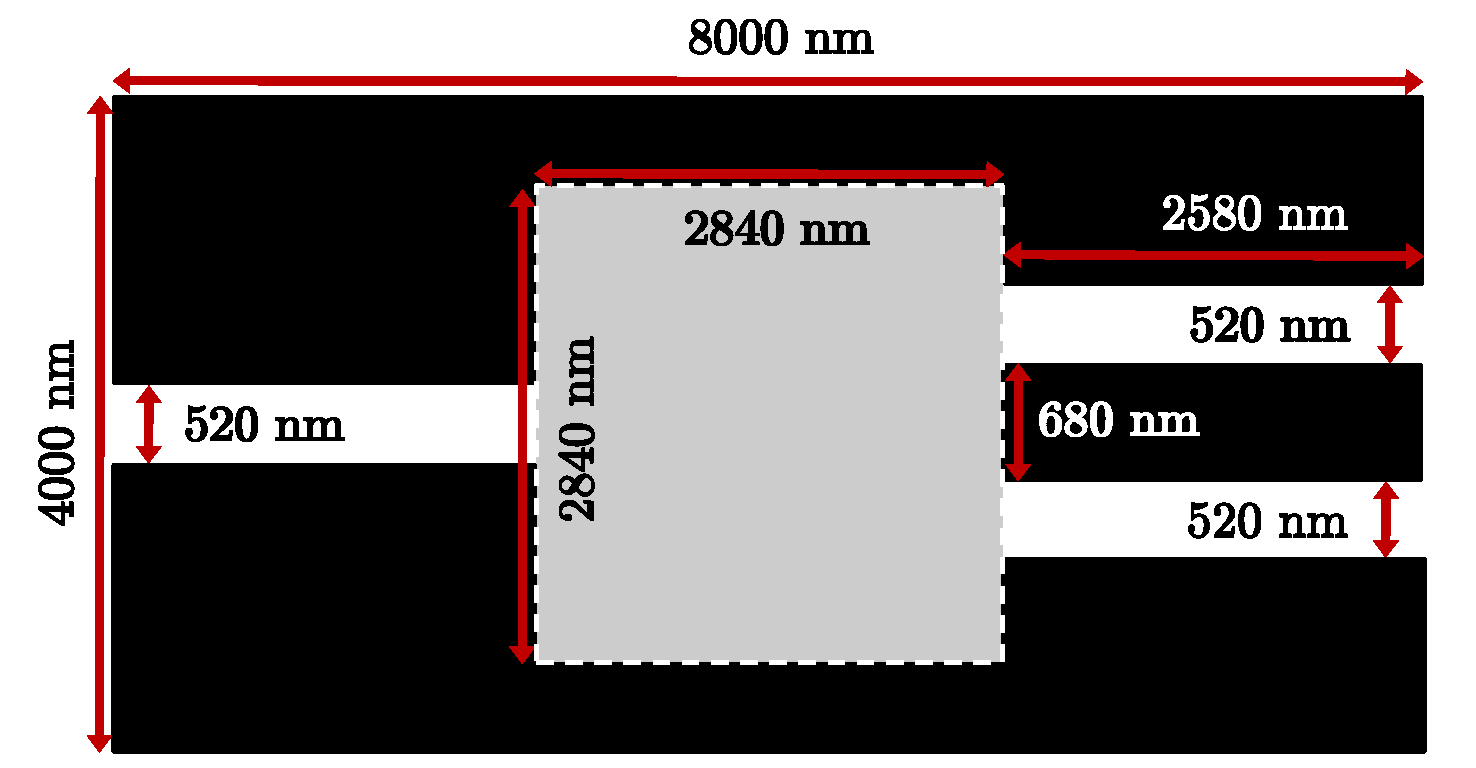
\includegraphics[width=0.7\textwidth]
    {fig/design/initialBox.pdf}
    \caption{Initial box structure dimensions, top-down view. The \texttt{design domain} is bordered by the dashed line.}
    \label{fig:initialBox}
\end{figure}

\begin{figure}[h!]
    \centering
    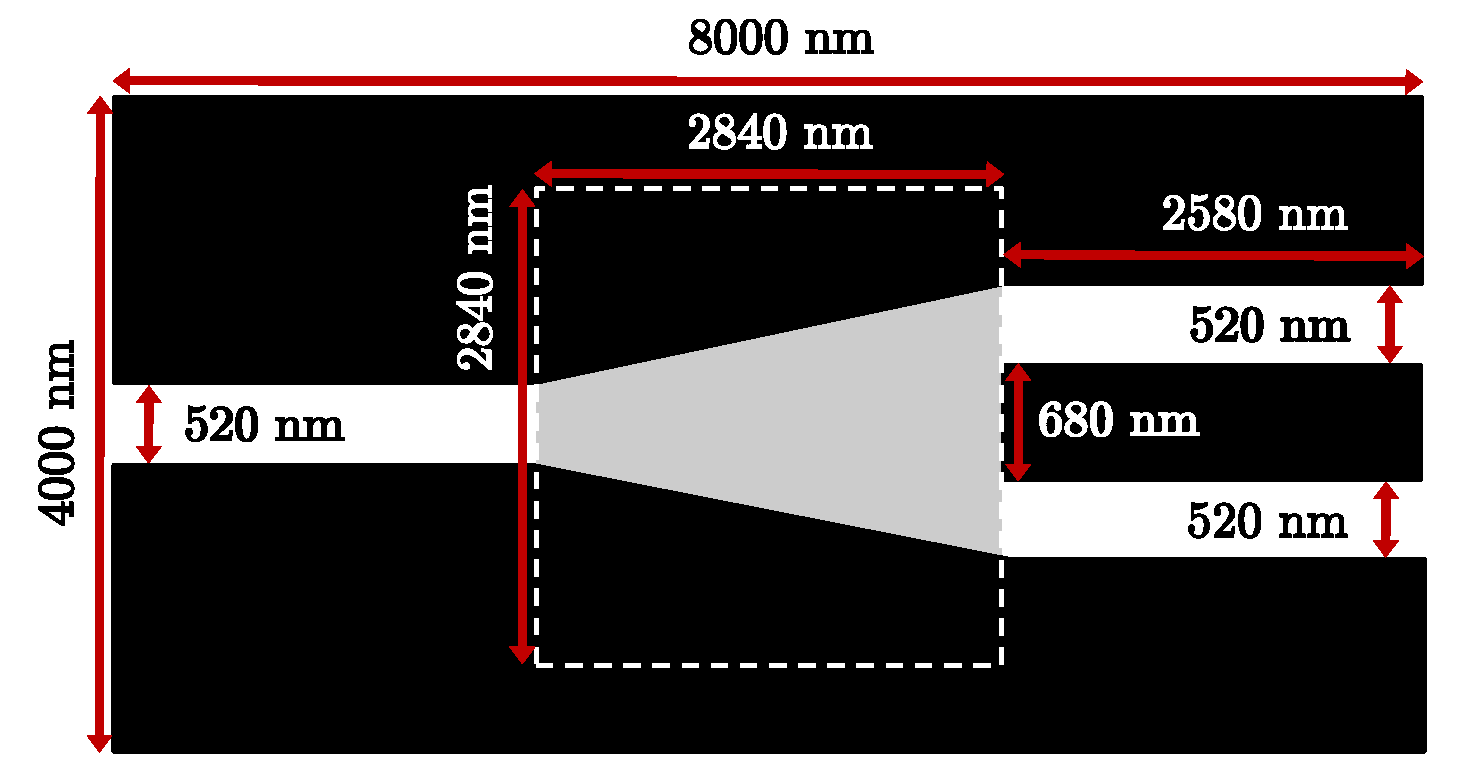
\includegraphics[width=0.7\textwidth]
    {fig/design/initialYjunction.pdf}
    \caption{Initial Y-junction structure dimensions, top-down view. The \texttt{design domain} bordered by the dashed line is the same as in the box structure, letting the software add silicon around the Y-junction and thereby not restricting the final structure to the dimensions of our initial structure.}
    \label{fig:initialYjunction}
\end{figure}

\begin{figure}[h!]
    \centering
    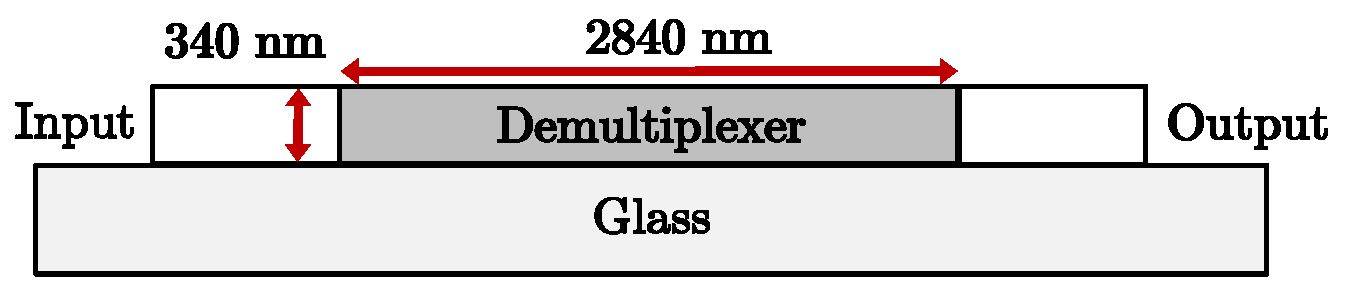
\includegraphics[width=0.7\textwidth]
    {fig/design/initialside.pdf}
    \caption{Initial structure dimensions, side-view. Left: input waveguide. Center: Demultiplexer, with an initial structure as a box or Y-junction. Right: Output waveguides.}
    \label{fig:initialside}
\end{figure}

\subsection{Objective functions}
When optimising a structure through the FDTD method with PhaZor, the user must choose an objective. The overall goal is clear: Demultiplex wavelengths of 1300 nm and 1550 nm into two separate output terminals while keeping their Gaussian form. But which objective best describes this goal? The objectives are communicated to PhaZor using \texttt{objective functions}. We used two such functions. The light sources implemented were two Gaussian pulses separated in time; a pulse centered at 1300 nm peaking at $t_1= 50$ fs, and a pulse centered at 1550 nm peaking at $t_2 = 1050$ fs, both with standard deviation $\sigma=\SI{10}{fs}$. We requested a structure that directed the entire pulse excited at $t_1$ to the upper output waveguide, and the entire pulse excited at $t_2$ to the lower output waveguide, see Fig. \ref{fig:initialBox}. While the pulses are separated in time during the optimisation for computational reasons, the fabricated structure can physically handle simultaneous pulses. While the goal seems straight-forward, we employed two very different approaches:\\

\textbf{The objective function \texttt{PointCustom SignalShape}} optimises for a Gaussian pulse with a certain amplitude $A$, peak time $t_0$, and temporal width $T$. This allows us to optimise for the first pulse (1300 nm) in the upper waveguide and second pulse (1550 nm) in the lower waveguide, as illustrated in Fig. \ref{fig:objectiveFunctionGaussian}. We set $A=0.1350$ (arbitrary units) and $t_0=\SI{128}{fs}$ 1580 nm into the upper waveguide and correspondingly $A=0.1235$ and $t_0 = \SI{1128}{fs}$ in the lower waveguide; for both waveguides, we set $T = 10$ fs. These values were obtained from running simulations in a \SI{8000}{nm} long waveguide (equal to the length of our demultiplexer structure) and recording the pulses at the corresponding position. This method yielded mediocre results, perhaps because the pulses tend to be delayed when traveling through the demultiplexer rather than an empty waveguide. The fact that the algorithm has to optimise for many constraints may also have been an obstacle. \\

\begin{figure}[h!]
    \centering
    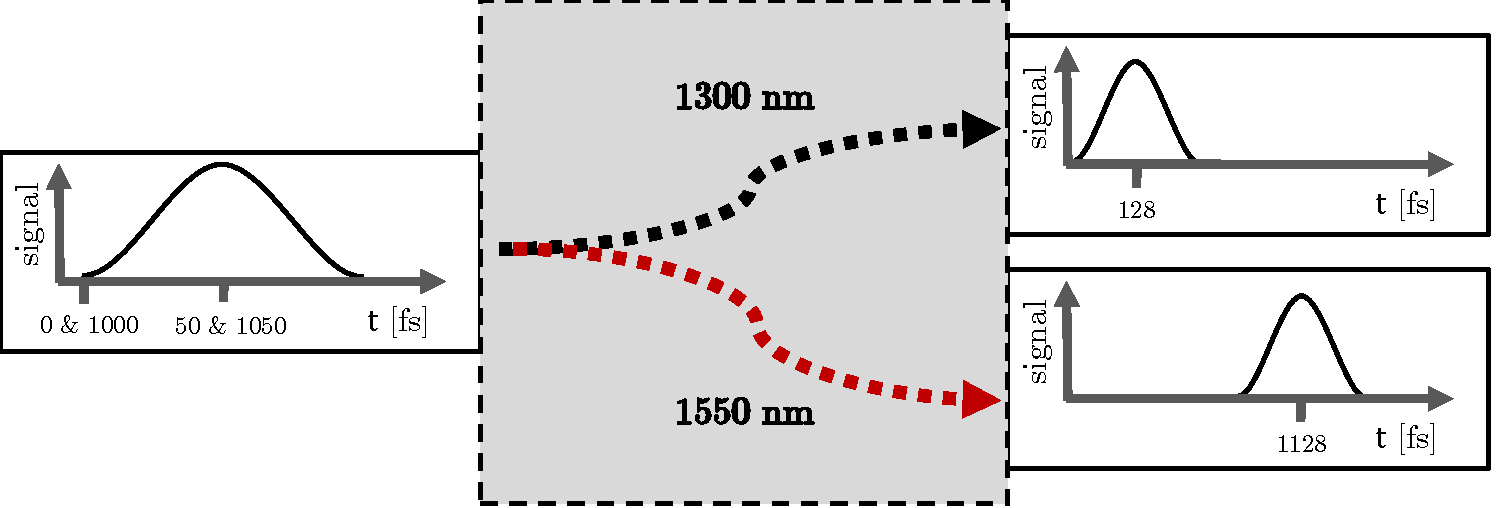
\includegraphics[width=1.0\textwidth]
    {fig/design/objectivefunctionsgaussian.pdf}
    \caption{When using the objective function \texttt{PointCustom SignalShape}, the main goal is the amplitude, peak time, and temporal shape of the output signals. The pulse sent at $t=0$ has a peak wavelength at 1300 nm. The pulse sent at $t= 1000$ fs has a peak wavelength at 1550 nm.}
    \label{fig:objectiveFunctionGaussian}
\end{figure}

\vspace{1cm}

\textbf{The objective function} \texttt{PointEnergyDensity}
optimises for a Gaussian power spectrum at a specified location with a given peak frequency $\nu$ and spectral width $d\nu$. We optimised for $\nu = 230.0$ THz ($\lambda =$ 1300 nm) and $ \nu= 193.4$ THz ($\lambda =$ 1550 nm) into the upper and lower output waveguide, respectively, and set $d\nu = 9.5$ THz for both waveguides. This is illustrated in Fig. \ref{fig:objectiveFunctionPED}.
This gave much better results. In hindsight, it makes sense: In each iteration, the structure is altered so that more power is delivered to e.g. the upper output, without specifying \textit{when} the signal should arrive. This may lead to odd signal shapes during the optimisation due to unpredictably bad local solutions, but after many (say, $\approx 70$) iterations, a good local solution has been obtained: a structure that splits wavelengths of 1300 nm and 1550 nm into two separate output terminals while keeping their Gaussian form.
 
\vspace{1cm}
 
\begin{figure}[h!]
    \centering
    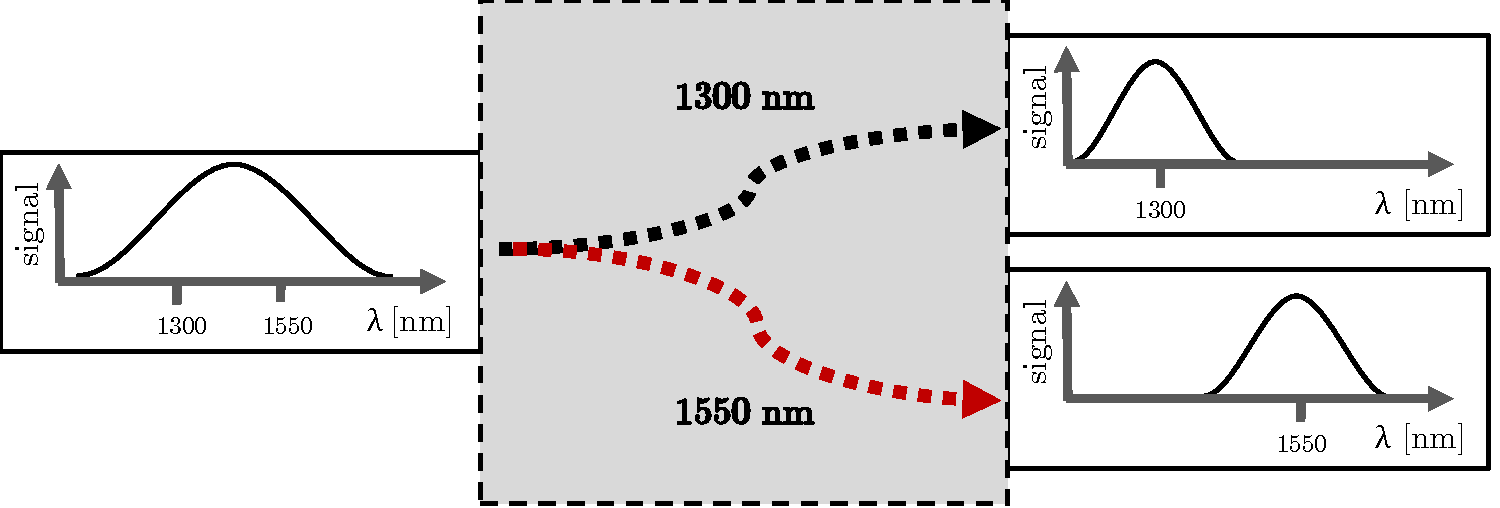
\includegraphics[width=1.0\textwidth]
    {fig/design/objectivefunctionsped.pdf}
    \caption{When using the objective function \texttt{PointEnergyDensity}, the main goal is optimising power at a specified spectral range. The pulse sent at $t=0$ has a peak wavelength at 1300 nm. The pulse sent at $t= 1000$ fs has a peak wavelength at 1550 nm.}
    \label{fig:objectiveFunctionPED}
\end{figure}
\vspace{1cm}

\subsection{Filter sizes}

In the PhaZor script, the filter size (more specifically, the  \texttt{filter radius}) is specified. This filter size limits the minimum feature size of which the software is allowed to redistribute material. Phazor uses preset sensitivity parameters to control whether material should stay or be moved. The filter starts out very light, letting the structure contain data points with properties between those of Si and air. Throughout the time steps, the filter strength increases exponentially, limiting the amount of material composed partially of Si and air, resulting in a structure mainly with data points representing pure Si or air. \\

The initial areas composed of a mixture of Si and air is visualised as a shaded area with the nuance describing the concentration level of Si. If the filter size is too large, meaning the task set by the objective functions cannot be fulfilled, the resulting design will still have shaded areas, because of the sensitivity and importance of these areas.
\vspace{1cm}
